\section{Factory method pattern}
  \label{sec:factory-method}
  
  Ya hicimos tests e implementamos los tipos de \textit{Bakémon} que queríamos, nos falta el último
  paso del TDD: refactorizar.

  Comencemos con la siguiente pregunta: ¿Existen los Bakémon sin tipo?
  Podría ser, pero en la manera que estamos modelando el juego no tiene mucho sentido.
  ¿De qué nos sirve entonces la clase \textit{Bakémon}?
  La verdad es que la estamos usando solamente para agrupar distintos tipos concretos de 
  \textit{Bakémon}.
  En otras palabras, \texttt{Bakemon} no tiene sentido como una clase.

  Transformemos la clase \texttt{Bakemon} en una interfaz.

  \begin{kotlin}
    interface Bakemon {
      val name: String
      val health: Int
      val level: Int
      val attack: Int
    }
  \end{kotlin}

  Y ahora modifiquemos las clases concretas para que implementen la interfaz \texttt{Bakemon}.

  \begin{kotlin}
    class FireBakemon(
      override val name: String,
      override val health: Int,
      override val level: Int,
      override val attack: Int
    ) : Bakemon {...}
  \end{kotlin}

  \begin{kotlin}
    class WaterBakemon(
      override val name: String,
      override val health: Int,
      override val level: Int,
      override val attack: Int
    ) : Bakemon {...}
  \end{kotlin}

  Noten que agregamos la palabra reservada \mintinline{kotlin}|override| a los atributos de las 
  clases concretas.
  Esto es porque los atributos de las interfaces son \textit{abstractos} por defecto, y por lo tanto
  deben ser sobreescritos en las clases que implementan la interfaz.

  Ahora, borremos el archivo \texttt{BakemonTest.kt} ya que nuestro cambio de diseño rompió los
  tests y no tiene sentido mantenerlos.

  Probemos que los tests sigan pasando y hagamos \textit{commit}.

  \begin{powershell}
    git add .
    git commit -m "REFACTOR Changes Bakemon class to an interface"
  \end{powershell}

  No hay mucho más que hacer para nuestros tipos de \textit{Bakémon}, pero notarán que los tests que
  escribimos para las clases de \textit{Bakémon} son muy similares.
  ¿Hay alguna forma de reusar ese código?
  La respuesta es que sí, pero primero debemos solucionar un problema importante.

  Veamos qué es lo que cambia entre los tests de las clases de \textit{Bakémon}.
  En todos los tests, creamos un objeto de la clase que estamos probando, y luego comparamos
  el objeto creado con otro objeto creado con los mismos parámetros.
  Noten que lo único que cambia entre los tests es el tipo de \textit{Bakémon} que estamos
  probando.
  En otras palabras, estamos concretizando la interfaz \texttt{Bakemon} en cada test.

  ¿Cómo podemos hacer para mantener la abstracción de la interfaz \texttt{Bakemon} en los tests?

  La respuesta nace del origen del problema, el constructor de las clases concretas.
  Cuando usamos un constructor estamos acoplando\footnote{Explicar significado de acoplar} nuestro código a una implementación concreta en
  lugar de una abstracción.
  Nos gustaría tener una manera genérica de crear objetos de la interfaz \texttt{Bakemon}.
  ¿Cómo podemos hacer eso?

  ¡Vamos con nuestro primer patrón de diseño\index{Patrón de diseño}!

  \begin{defaultbox}[Factory method pattern]
    \index{Factory method pattern}
    \textbf{Problema:} \textit{Necesito una manera de crear objetos de una interfaz sin acoplar
    mi código a una implementación concreta.}

    \textbf{Solución:} \textit{Definir una interfaz para crear objetos, pero dejar que las
    subclases decidan qué clase concreta instanciar.}
  \end{defaultbox}

  El patrón \textit{factory method} es un patron de diseño creacional\index{Patrón de 
  diseño creacional} que nos permite reusar los constructores de clases concretas mediante la
  abstracción del proceso de creación.

  \begin{figure}[ht!]
    \centering
    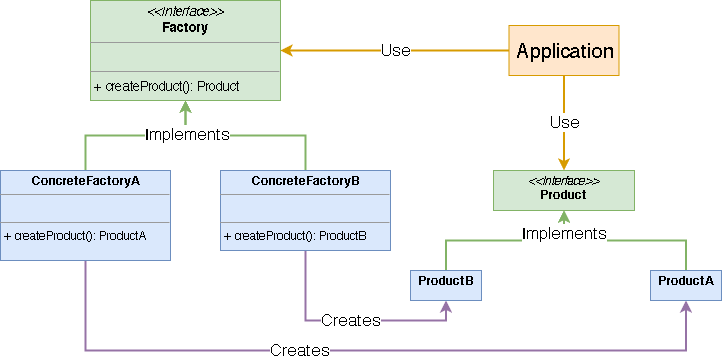
\includegraphics[width=0.8\textwidth]{img/oop/factory/abstract_factory.png}
    \caption{Estructura del patrón de diseño \textit{Factory Method}}
    \label{fig:abstract_factory}
  \end{figure}

  La \cref{fig:abstract_factory} muestra la estructura del patrón de diseño \textit{Abstract 
  Factory}.
  Veamos como adaptar esto a nuestro problema.
  Pero primero: ¿Que es un patrón de diseño?

  \begin{defaultbox}[Patrón de diseño]
    \index{Patrón de diseño}
    Un patrón de diseño es una solución general a un problema recurrente en el diseño de software.    
  \end{defaultbox}

  \begin{center}
    ¿Así como un algoritmo?
  \end{center}

  No, un patrón de diseño no es un algoritmo.
  Un algoritmo define una serie de pasos para solucionar un problema particular.
  Un patrón de diseño por otro lado define una estructura general para modelar una solución.
  Esto significa que la implementación concreta de un patrón de diseño puede variar de acuerdo a
  las necesidades del problema.
  
  Ahora sí, veamos como adaptar el patrón de diseño \textit{Factory Method} a nuestro problema.
  Lo primero que debemos definir es cuál es la familia de objetos que queremos crear.
  En nuestro caso, la familia de objetos que queremos crear son los tipos de \textit{Bakémon}.
  Luego, debemos definir la interfaz que va a proveer la creación de los objetos de la familia, en
  nuestro caso, una interfaz \texttt{BakemonFactory}.
  Por último, debemos definir cuáles son los métodos que va a tener la interfaz 
  \texttt{BakemonFactory}, en nuestro caso, sólo necesitamos un método, ya que cada tipo de
  fábrica va a crear un tipo de \textit{Bakémon}.

  Veamos cómo implementar esto en código.
  Comencemos por definir la interfaz \texttt{BakemonFactory}, para esto, vamos a crear un nuevo
  paquete llamado \url{cl.ravenhill.bakemon.factory} y dentro de ese paquete vamos a crear una nueva
  interfaz llamada \texttt{BakemonFactory}.  

  \begin{kotlin}
    interface BakemonFactory {
      fun createBakemon(name: String, health: Int, level: Int, attack: Int): Bakemon
    }
  \end{kotlin}

  Luego, debemos definir las clases concretas que implementan la interfaz \texttt{BakemonFactory}.
  Comencemos por los tests:

  \begin{kotlin}
    class FireBakemonFactoryTest : FunSpec({
      val name = "Karmander"
      val health = 25
      val level = 5
      val attack = 4
      
      lateinit var factory: BakemonFactory

      beforeTest {
        factory = FireBakemonFactory()
      }

      test("A FireBakemon should be created") {
        val bakemon = factory.createBakemon(name, health, level, attack)
        bakemon.name shouldBe name
        bakemon.health shouldBe health
        bakemon.level shouldBe level
        bakemon.attack shouldBe attack
      }
    })
  \end{kotlin}

  \begin{kotlin}
    class WaterBakemonFactoryTest : FunSpec({
      val name = "Kokodile"
      val health = 25
      val level = 5
      val attack = 4
      
      lateinit var factory: BakemonFactory

      beforeTest {
        factory = WaterBakemonFactory()
      }

      test("A WaterBakemon should be created") {
        val bakemon = factory.createBakemon(name, health, level, attack)
        bakemon.name shouldBe name
        bakemon.health shouldBe health
        bakemon.level shouldBe level
        bakemon.attack shouldBe attack
      }
    })
  \end{kotlin}

  \begin{ejercicio}{Bakémon}
    Implemente los tests para la clase \texttt{GrassBakemonFactory}.
  \end{ejercicio}
  
  Bien, ahora que tenemos los tests, podemos implementar las clases concretas que implementan la
  interfaz \\\texttt{BakemonFactory}.

  \begin{kotlin}
    class FireBakemonFactory : BakemonFactory {
      override fun createBakemon(name: String, health: Int, level: Int, attack: Int) =
        FireBakemon(name, health, level, attack)
    }
  \end{kotlin}

  \begin{kotlin}
    class WaterBakemonFactory : BakemonFactory {
      override fun createBakemon(name: String, health: Int, level: Int, attack: Int) =
        WaterBakemon(name, health, level, attack)
    }
  \end{kotlin}

  Ahora corremos los tests y vemos que todo funciona como esperábamos.
  Con esto podemos hacer \textit{commit} a nuestros cambios.

  \begin{powershell}
    git add .
    git commit -m "FEAT Implements Factory Method pattern"
  \end{powershell}
